\documentclass[12pt,a4paper,twoside,openright]{report}
\let\openright=\cleardoublepage



%%% Choose a language %%%

\newif\ifEN
\ENtrue   % uncomment this for english
%\ENfalse   % uncomment this for czech

%%% Configuration of the title page %%%

\newif\ifMFF
%\MFFtrue % comment this out for the version with a big UK university logo
\def\UKName{Charles University in Prague} %this is used in UK-logo-version
\def\UKFaculty{Faculty of Science}
\def\ThesisTypeName{\ifEN BACHELOR THESIS \else BAKALÁŘSKÁ PRÁCE \fi}
%\def\ThesisTypeName{\ifEN MASTER THESIS \else DIPLOMOVÁ PRÁCE \fi}
%\def\ThesisTypeName{\ifEN RIGOROUS THESIS \else RIGORÓZNÍ PRÁCE \fi}
%\def\ThesisTypeName{\ifEN DOCTORAL THESIS \else DISERTAČNÍ PRÁCE \fi}
\def\SupervisedThesisName{\ifEN bachelor \else bakalářské \fi}
%\def\SupervisedThesisName{\ifEN master \else diplomové \fi}
%\def\SupervisedThesisName{\ifEN rigorous \else rigorózní \fi}
%\def\SupervisedThesisName{\ifEN doctoral \else disertační \fi}


%%% Fill in your details %%%

% (Note: \xxx is a "ToDo label" which makes the unfilled visible. Remove it.)
\def\ThesisTitle{The influence of non-domain regions' composition on the activity of multi-domain protein kinases}
\def\ThesisAuthor{Jan Hamalčík}
\def\YearSubmitted{2020}

% department assigned to the thesis
\def\Department{Department of Cell Biology}
% Is it a department (katedra), or an institute (ústav)?
\def\DeptType{Department}

\def\Supervisor{doc. RNDr. Jiří Vondrášek, CSc.}
\def\SupervisorsDepartment{Institute of Organic Chemistry and Biochemistry of the CAS}

% Study programme and specialization
\def\StudyProgramme{Bioinformatics}
\def\StudyBranch{Bioinformatics}

\def\Dedication{%
Dedication. \xxx{It is nice to say thanks to supervisors, friends, family, book authors and food providers.}
}

\def\Abstract{%
\xxx{Abstracts are an abstract form of art. Use the most precise, shortest sentences that state what problem the thesis addresses, how it is approached, pinpoint the exact result achieved, and describe the applications and significance of the results. Highlight anything novel that was discovered or improved by the thesis. Maximum length is 200 words, but try to fit into 120. Abstracts are often used for deciding if a reviewer will be suitable for the thesis; a well-written abstract thus increases the probability of getting a reviewer who will like the thesis.}
% ABSTRACT IS NOT A COPY OF YOUR THESIS ASSIGNMENT!
}

% 3 to 5 keywords (recommended), each enclosed in curly braces.
% Keywords are useful for indexing and searching for the theses by topic.
\def\Keywords{%
{protein domains}, {multi-domain proteins}, {protein function}, {non-domain regions}, {protein kinases}
}

% If your abstracts are long and do not fit in the infopage, you can make the
% fonts a bit smaller by this setting. (Also, you should try to compress your abstract more.)
% Alternatively, consider increasing the size of the page by uncommenting the
% geometry modification in thesis.tex.
\def\InfoPageFont{}
%\def\InfoPageFont{\small}  %uncomment to decrease font size

\ifEN\relax\else
% If you are writing a czech thesis, you additionally need to fill in the
% english translation of the metadata here!
\def\ThesisTitleEN{\xxx{Thesis title in English}}
\def\DepartmentEN{\xxx{Name of the department in English}}
\def\DeptTypeEN{\xxx{Department}}
\def\SupervisorsDepartmentEN{\xxx{Superdepartment}}
\def\StudyProgrammeEN{\xxx{study programme}}
\def\StudyBranchEN{\xxx{study branch}}
\def\AbstractEN{%
\xxx{Abstract.}
}
\def\KeywordsEN{%
\xxx{{key} {words}}
}
\fi


\usepackage[a-2u]{pdfx}

\ifEN\else\usepackage[czech,shorthands=off]{babel}\fi
\usepackage[utf8]{inputenc}
\usepackage[T1]{fontenc}

% See https://en.wikipedia.org/wiki/Canons_of_page_construction before
% modifying the size of printable area. LaTeX defaults are great.
% If you feel it would help anything, you can enlarge the printable area a bit:
%\usepackage[textwidth=390pt,textheight=630pt]{geometry}
% The official recommendation expands the area quite a bit (looks pretty harsh):
%\usepackage[textwidth=145mm,textheight=247mm]{geometry}

%%% FONTS %%%
%\usepackage{lmodern} % TeX "original" (this sets up the latin mono)

% Optionally choose an override for the main font for typesetting
%\usepackage[mono=false]{libertinus} % popular for comp-sci (ACM uses this)
%\usepackage{tgschola} % Schoolbook-like (gives a bit of historic feel)
%\usepackage[scale=0.96]{tgpagella} % Palladio-like (popular in formal logic).

% Optionally choose a custom sans-serif fonts (e.g. for figures and tables).
% Default sans-serif font is usually Latin Modern Sans. Some font packages
% (e.g. libertinus) replace that with a better matching sans-serif font.
%\usepackage{tgheros} % recommended and very readable (Helvetica-like)
%\usepackage{FiraSans} % looks great
% DO NOT typeset the main text in sans-serif font!
% The serifs make the text easily readable on the paper.

% IMPORTANT FONT NOTE: Some fonts require additional PDF/A conversion using
% the pdfa.sh script. These currently include only 'tgpagella'; but various
% other fonts from the texlive distribution need that too (mainly the Droid
% font family).


% some useful packages
\usepackage{amsmath,amsfonts,amsthm,bm}
\usepackage{graphicx}
\usepackage{xcolor}
\usepackage{booktabs}
\usepackage{float}
\usepackage{longtable}

% load bibliography tools
\usepackage[backend=bibtex,natbib,style=ext-numeric-comp,sorting=none]{biblatex}
% alternative with alphanumeric citations (more informative than numbers):
%\usepackage[backend=bibtex,natbib,style=alphabetic]{biblatex}
%
% alternatives that conform to iso690
% (iso690 is not formally required on MFF, but may help elsewhere):
%\usepackage[backend=bibtex,natbib,style=iso-numeric]{biblatex}
%\usepackage[backend=bibtex,natbib,style=iso-alphabetic]{biblatex}
%
% additional option choices:
%  - add `giveninits=true` to typeset "E. A. Poe" instead of full Edgar Allan
%  - add `maxnames=10` to limit (or loosen) the maximum number of authors in
%    bibliography entry before shortening to `et al.` (useful when referring to
%    book collections that may have hundreds of authors)
%  - for additional flexibility (e.g. multiple reference sections, etc.),
%    remove `backend=bibtex` and compile with `biber` instead of `bibtex` (see
%    Makefile)
%
% possibly reverse the names of the authors with the default styles:
%\DeclareNameAlias{default}{family-given}

% load the file with bibliography entries
\addbibresource{refs}

% remove this if you won't use fancy verbatim environments
\usepackage{fancyvrb}

% remove this if you won't typeset TikZ graphics
\usepackage{tikz}
\usetikzlibrary{positioning} %add libraries as needed (shapes, decorations, ...)

% remove this if you won't typeset any pseudocode
\usepackage{algpseudocode}
\usepackage{algorithm}

% remove this if you won't list any source code
\usepackage{listings}


\hypersetup{unicode}
\hypersetup{breaklinks=true}

\usepackage[noabbrev]{cleveref}

\input{todos} % remove this before compiling the final version


% use this for typesetting a chapter without a number, e.g. intro and outro
\def\chapwithtoc#1{
\chapter*{#1}
\addcontentsline{toc}{chapter}{\protect\numberline{}#1}
}

\def\secwithtoc#1{
\section*{#1}
\addcontentsline{toc}{section}{\protect\numberline{}#1}
}

\def\subsecwithtoc#1{
\subsection*{#1}
\addcontentsline{toc}{subsection}{\protect\numberline{}#1}
}

% \def\secwithtoc#1{
% \section*{#1}
% \addcontentsline{toc}{section}{\protect\numberline{}#1}
% }
%
% \def\subsecwithtoc#1{
% \subsection*{#1}
% \addcontentsline{toc}{subsection}{\protect\numberline{}#1}
% }

% If there is a line/figure overflowing into page margin, this will make the
% problem evident by drawing a thick black line at the overflowing spot. You
% should not disable this.
\overfullrule=3mm

% The maximum stretching of a space. Increasing this makes the text a bit more
% sloppy, but may prevent the overflows by moving words to next line.
\emergencystretch=1em

\ifEN
\theoremstyle{plain}
\newtheorem{thm}{Theorem}
\newtheorem{lemma}[thm]{Lemma}
\newtheorem{claim}[thm]{Claim}
\newtheorem{defn}{Definition}
\theoremstyle{remark}
\newtheorem*{cor}{Corollary}
\else
\theoremstyle{plain}
\newtheorem{thm}{Věta}
\newtheorem{lemma}{Lemma}
\newtheorem{claim}{Tvrzení}
\newtheorem{defn}{Definice}
\theoremstyle{remark}
\newtheorem*{cor}{Důsledek}
\fi

\newenvironment{myproof}{
  \par\medskip\noindent
  \textit{\ifEN Proof \else Důkaz \fi}.
}{
\newline
\rightline{$\qedsymbol$}
}

% real/natural numbers
\newcommand{\R}{\mathbb{R}}
\newcommand{\N}{\mathbb{N}}

% asymptotic complexity
\newcommand{\asy}[1]{\mathcal{O}(#1)}

% listings and default lstlisting config (remove if unused)
\floatstyle{ruled}
\newfloat{listing}{tbp}{lst}
\ifEN\floatname{listing}{Listing}
\else\floatname{listing}{Výpis kódu}\fi
\lstset{%
  language=C++,
  tabsize=2,
  showstringspaces=false,
  basicstyle=\footnotesize\tt\color{black!75},
  identifierstyle=\bfseries\color{black},
  commentstyle=\color{green!50!black},
  stringstyle=\color{red!50!black},
  keywordstyle=\color{blue!75!black}}

% re-styling of the captions with the float package
\makeatletter
\newcommand\floatc@plainb[2]{\setbox\@tempboxa\hbox{{\@fs@cfont #1} #2}%
\ifdim\wd\@tempboxa>\hsize {\@fs@cfont #1} #2\par
\else\hbox to\hsize{\hfil\box\@tempboxa\hfil}\fi}
\newcommand\fs@plainb{\def\@fs@cfont{\bfseries}\let\@fs@capt\floatc@plainb%
\def\@fs@pre{}\def\@fs@post{}%
\def\@fs@mid{\vspace\abovecaptionskip\relax}%
\let\@fs@iftopcapt\iffalse}
\makeatother
\floatstyle{plainb}
\restylefloat{table}
\restylefloat{figure}

% Czech versions of the used cleveref references (It's not as convenient as in
% English because of declension, cleveref is limited to sg/pl nominative. Use
% plain \ref to dodge that.)
\ifEN\relax\else
\crefname{chapter}{kapitola}{kapitoly}
\Crefname{chapter}{Kapitola}{Kapitoly}
\crefname{section}{sekce}{sekce}
\Crefname{section}{Sekce}{Sekce}
\crefname{subsection}{sekce}{sekce}
\Crefname{subsection}{Sekce}{Sekce}
\crefname{subsubsection}{sekce}{sekce}
\Crefname{subsubsection}{Sekce}{Sekce}
\crefname{figure}{obrázek}{obrázky}
\Crefname{figure}{Obrázek}{Obrázky}
\crefname{table}{tabulka}{tabulky}
\Crefname{table}{Tabulka}{Tabulky}
\crefname{listing}{výpis}{výpisy}
\Crefname{listing}{Výpis}{Výpisy}
\floatname{algorithm}{Algoritmus}
\crefname{algorithm}{algoritmus}{algoritmy}
\Crefname{algorithm}{Algoritmus}{Algoritmy}
\newcommand{\crefpairconjunction}{ a~}
\newcommand{\crefrangeconjunction}{ a~}
\fi
 % use this file for various custom definitions

\setlength\topmargin{0mm}
\setlength\headsep{0mm}
\setlength\headheight{0mm}
\setlength\textheight{247mm}


\begin{document}

% the layout is mandatory, edit only in dire circumstances

\pagestyle{empty}
\hypersetup{pageanchor=false}
\begin{center}

\ifMFF
\ifEN
\centerline{\mbox{
\includegraphics[width=166mm]{img/logo-en.pdf}}}
\else
\centerline{\mbox{
\includegraphics[width=166mm]{img/logo-cs.pdf}}}
\fi
\vspace{-8mm}
\else
{\large\noindent\UKName\par\medskip\par\UKFaculty }
\fi
\vfill

{\bf\Large\ThesisTypeName}

\vfill

\ifMFF\relax\else\includegraphics[width=70mm]{img/uklogo.pdf}

\vfill\fi

{\LARGE\ThesisAuthor}

\vspace{15mm}

{\LARGE\bfseries\ThesisTitle}

\vfill

\Department

\vfill

{
\centerline{\vbox{\halign{\hbox to 0.45\hsize{\hfil #}&\hskip 0.5em\parbox[t]{0.45\hsize}{\raggedright #}\cr
\ifEN Supervisor of the \SupervisedThesisName thesis:
\else Vedoucí \SupervisedThesisName práce: \fi
& \Supervisor \cr
\noalign{\vspace{2mm}}
\ifEN Study programme: \else Studijní program: \fi
& \StudyProgramme \cr
\noalign{\vspace{2mm}}
\ifEN Study branch: \else Studijní obor: \fi
& \StudyBranch \cr
}}}}

\vfill

\ifEN Prague \else Praha \fi
\YearSubmitted

\end{center}

\newpage

% remember to sign this!
\openright
\hypersetup{pageanchor=true}
\pagestyle{plain}
\pagenumbering{roman}
\vglue 0pt plus 1fill

\ifEN
\noindent
I declare that I carried out this bachelor thesis independently, and only with the cited
sources, literature and other professional sources. It has not been used to obtain another
or the same degree.
\else
\noindent
Prohlašuji, že jsem tuto bakalářskou práci vypracoval(a) samostatně a výhradně
s~použitím citovaných pramenů, literatury a dalších odborných zdrojů.
Tato práce nebyla využita k získání jiného nebo stejného titulu.
\fi

\ifEN
\medskip\noindent
I understand that my work relates to the rights and obligations under the Act No.~121/2000 Sb.,
the Copyright Act, as amended, in particular the fact that the Charles
University has the right to conclude a license agreement on the use of this
work as a school work pursuant to Section 60 subsection 1 of the Copyright~Act.
\else
\medskip\noindent
Beru na~vědomí, že se na moji práci vztahují práva a povinnosti vyplývající
ze zákona č. 121/2000 Sb., autorského zákona v~platném znění, zejména skutečnost,
že Univerzita Karlova má právo na~uzavření licenční smlouvy o~užití této
práce jako školního díla podle §60 odst. 1 autorského zákona.
\fi

\vspace{10mm}


\ifEN
\hbox{\hbox to 0.5\hsize{%
In \hbox to 6em{\dotfill} date \hbox to 6em{\dotfill}
\hss}\hbox to 0.5\hsize{\dotfill\quad}}
\smallskip
\hbox{\hbox to 0.5\hsize{}\hbox to 0.5\hsize{\hfil Author's signature\hfil}}
\else
\hbox{\hbox to 0.5\hsize{%
V \hbox to 6em{\dotfill} dne \hbox to 6em{\dotfill}
\hss}\hbox to 0.5\hsize{\dotfill\quad}}
\smallskip
\hbox{\hbox to 0.5\hsize{}\hbox to 0.5\hsize{\hfil Podpis autora\hfil}}
\fi

\vspace{20mm}
\newpage

% dedication

\openright

\noindent
\Dedication

\newpage

% mandatory information page

\openright

\vbox to 0.49\vsize{\InfoPageFont
\setlength\parindent{0mm}
\setlength\parskip{5mm}

\ifEN Title: \else Název práce: \fi
\ThesisTitle

\ifEN Author: \else Autor: \fi
\ThesisAuthor

\DeptType:
\Department

\ifEN Supervisor: \else Vedoucí bakalářské práce: \fi
\Supervisor, \SupervisorsDepartment

\ifEN Abstract: \else Abstrakt: \fi
\Abstract

\ifEN Keywords: \else Klíčová slova: \fi
\Keywords

\vss}\ifEN\relax\else\nobreak\vbox to 0.49\vsize{\InfoPageFont
\setlength\parindent{0mm}
\setlength\parskip{5mm}

Title:
\ThesisTitleEN

Author:
\ThesisAuthor

\DeptTypeEN:
\DepartmentEN

Supervisor:
\Supervisor, \SupervisorsDepartmentEN

Abstract:
\AbstractEN

Keywords:
\KeywordsEN

\vss}
\fi

\newpage

\openright
\pagestyle{plain}
\pagenumbering{arabic}
\setcounter{page}{1}


\tableofcontents

\chapwithtoc{List of Abbreviations}

\begin{longtable}[l]{ l l }
  2D & two-dimensional \\
  3D & three-dimensional \\
  ATP & adenosine triphosphate \\
  EC & Enzyme Commission \\
  GO & Gene Ontology \\
  GTP & guanosine triphosphate \\
  HMM & profile hidden Markov Model \\
  MSA & multiple sequence alignment \\
  pI & isoelectric point \\
  PK & protein kinase \\
  UMAP & Uniform Manifold Approximation and Projection \\
  UPR.dat & \texttt{uniprot\_reference\_proteomes.dat} \\
\end{longtable}

Throughout this thesis, the standard one and three letter codes for the L-amino acids will
be used.

\chapwithtoc{Introduction}
\label{intro}

\secwithtoc{Proteins and domains}
\label{intro:prodoms}

  Proteins are amino acid chains, polypeptides, that serve a variety of functions within
  living cells, including structural support and movement, interactions with cell's
  environment, and biochemical reaction catalysis~\cite{alberts2018molecular}.
  To function properly, proteins have to fold into their native conformation, and as
  demonstrated by \citet{anfinsen1961kinetics} on bovine pancreatic ribonuclease, the
  information for correct folding is contained in the amino acid sequence itself.

  Different sequences fold into different three-dimensional conformations.
  Certain local regions form secondary structures, such as $\alpha$-helices and
  $\beta$-sheets, and these locally ordered regions associate to form the whole protein,
  or in the case of some larger proteins, to form folding units~\cite{levitt1975computer}.
  If the folding units would be stable, given that the polypeptide chain connecting them
  to the rest of the protein molecule were to be cleaved, these subassemblies can be
  referred to as \emph{domains}~\cite{goldberg1969tertiary, levitt1975computer}.
  Nevertheless, today's definition requires that these subassemblies also conceivably
  function in isolation, and members of the same \emph{domain family} tend to possess an
  ancient evolutionary relationship and often a similar
  function~\cite{ponting2002natural}.

  Many bioinformatics tools are available online to perform domain identification within
  a protein sequence.
  The \emph{SCOP} database organizes proteins of known three-dimensional structures
  according to their evolutionary and structural relationship~\cite{murzin1995scop}.
  It classifies non-redundant protein domains and defines them on two main levels of SCOP
  classification, family and superfamily.
  The designation of proteins in SCOP has been constructed mainly
  manually~\cite{andreeva2020scop}.

  Other tools tend to implement semimanual approaches, typically including a
  \emph{profile hidden Markov Model} (HMM), a powerful probabilistic method describing the
  sequence conservation in a family~\cite{krogh1994hidden, eddy1996hidden}.
  \emph{Pfam}~\cite{sonnhammer1997pfam} is such an example.
  Each protein family in Pfam database consists of a seed alignment forming the basis to
  build a HMM-based profile~\cite{el2019pfam} by engaging the HMMER
  software~\cite{finn2010pfam, finn2011hmmer}.
  Another protein structure classification database using HMMs to scan protein sequences
  against it is called \emph{CATH}~\cite{dawson2017cath}.
  CATH clusters proteins on four main levels, class (C), architecture (A), topology (T),
  and homologous superfamily (H)~\cite{orengo1997cath}.
  CATH, Pfam, and many more, are then integrated in a general resource for protein
  families, domains, and functional sites, called InterPro~\cite{finn2017interpro}.
  The authors aim to create a non-redundant characterization, and the software package
  InterProScan provides an interface to functionally classify novel nucleotide or protein
  sequences~\cite{zdobnov2001interproscan}.
  By uniting member databases, InterPro exploits their individual strengths, thus
  significantly contributing in the troublesome effort of automatic
  annotation~\cite{apweiler2000interpro}.

  \citet{chothia1992one} predicted that there is a limited number of protein families
  nature uses in evolution.
  Later, \citet{wolf2000estimating} estimated the sum to be between 4,000 and 7,000, and
  the Pfam database seems to confirm this calculation, as it records 6,248 family entries
  in release 32.0~\cite{el2019pfam}.

\secwithtoc{Protein kinase family}
\label{intro:pkinase}

  \begin{figure}
    \centering
    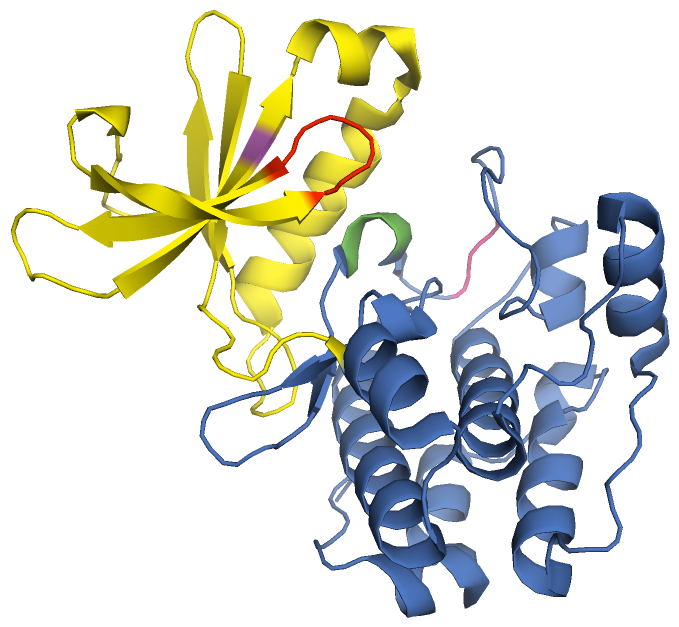
\includegraphics[width=0.8\linewidth]{img/aurora.png}
    \caption{The bilobal structure of the protein kinase domain from the Aurora A protein
    kinase.
    Structure downloaded from the PDBe, entry code 4dee~\cite{lawrence2012development},
    visualized with the PyMOL Molecular Graphics System~\cite{PyMOL}.
    Yellow: The small lobe.
    Blue: The large lobe.
    Red: Gly-X-Gly-X-X-Gly motif.
    Magenta: The invariant lysine.
    Green: DFG motif.
    Pink: APE motif.
    }
    \label{fig:aurora}
  \end{figure}

  An example of a protein family is the \emph{protein kinase family}, labeled as
  \texttt{PF00069} is the Pfam database.
  It is large and diverse~\cite{hanks1988protein, hunter19911}, and generally, protein
  kinases are involved in most of the signal transduction in eukaryotic cells.
  They control a variety of cellular processes, among other things metabolism, cell cycle
  progression, differentiation, transcription, cell movement, communication, and
  apoptosis~\cite{kemp2003amp, matsuoka1998linkage, johnson1994sequential,
  vermeulen2003transcriptional, chen1994cell, warn1998regulation, cross2000serine}.
  As protein kinases function as a responsive regulatory system, it is not surprising that
  their turnover rate is rather fast, with a half-life averaging less than an
  hour~\cite{hunter1982phosphotyrosine}.
  And because kinase activity at the wrong place or at the wrong time can lead to
  unfavorable cell transformation and cancer~\cite{koivunen2006protein,
  caretta2011protein}, they are a fascinating subject in molecular biology and
  bioinformatics.

  The conformational space of protein kinase domains is conserved~\cite{ung2018redefining}
  with common structural features specific to the protein kinase
  family~\cite{taylor1994three}.
  The enzyme structure is bilobal.
  The smaller lobe on the N-terminus is composed of a five-stranded antiparallel
  $\beta$-sheet and one $\alpha$-helix~\cite{knighton1991crystal} called $\alpha$C, which
  takes part in the stabilization of the active
  conformation~\cite{mobitz2015abc, huse2002conformational}.
  The broadly helical larger lobe associated with the C-terminus adds up to have seven
  $\alpha$-helices and one antiparallel $\beta$-sheet placed on the surface of the cleft
  between the two lobes, where the catalytic site is
  located~\cite{knighton1991crystal, taylor1994three, azam2008activation}.
  Twelve major subdomains can be further recognized throughout the protein kinase
  family~\cite{hanks1988protein, hanks19912, hanks1995eukaryotic}.

  Multiple sequence alignments of domains from the protein kinase family uncover many
  highly conserved residues and motifs, some of which are strictly required for the kinase
  activity.
  The nucleotide binding consensus sequence Gly-X-Gly-X-X-Gly is found in subdomain I and
  contains the first, second, and third essential glycine.
  Any side chain at glycines' positions would interfere with the incoming ATP (or GTP).
  The whole motif turns sharply around the nucleotide, with the first essential glycine
  being in contact with ribose, while the second provides space for the pyrophosphate
  group~\cite{wierenga1983predicted, hanks1988protein}.
  The $\beta$-phosphate moiety's oxygens are hydrogen bonded with the backbone amides of
  residues around the third fundamental glycine, and side chains surrounding this motif
  contribute to the hydrophobic pocket for the adenine ring of
  ATP~\cite{hanks1995eukaryotic}.
  GTP can be utilized as well, however, ATP will always have a lower Michaelis constant
  $\mathrm{K_{m}}$~\cite{hunter1985protein}.
  Regardless which, the phosphate donor is bound as a complex together with a divalent
  cation, with $\mathrm{Mn^{2+}}$ usually preferred over $\mathrm{Mg^{2+}}$ and
  others~\cite{witte1980abelson, richert1979characterization, wong1984purification}.

  An invariant lysine in subdomain II corresponding to PKA-C$\alpha$ Lys72 is thought to
  be the best characterized catalytic domain residue~\cite{hanks1988protein}.
  It forms a salt bridge with the carboxyl group of the practically invariant glutamate in
  subdomain III, which stabilizes the interactions between the lysine and the $\alpha$-
  and $\beta$-phosphates of ATP~\cite{hanks1995eukaryotic}.
  As \citet{kamps1986neither} showed in their work on p60\textsuperscript{\textit{src}}
  tyrosine protein kinase, all substitutions of the lysine, including arginine and
  histidine, result in loss of protein kinase activity.

  Highly conserved triad Asp-Phe-Gly (DFG) can be found in subdomain VII.
  It is part of the so called activation loop and helps orient the $\gamma$-phosphate of
  the ATP for transfer~\cite{hanks1995eukaryotic}.
  The activation loop is centrally located and provides a platform for a peptide
  substrate by interacting with the
  $\alpha$C-helix~\cite{huse2002conformational, mobitz2015abc}.
  Autophosphorylation of three conserved tyrosines within the activation loop results in
  an active kinase state, unphosphorylated loop traverses through the cleft between
  the two lobes of the kinase domain, thus yielding both protein substrate and ATP binding
  sites inaccessible~\cite{hubbard1997crystal}.
  The recognition of peptide substrates in the active state is then mediated by the
  Ala-Pro-Glu (APE) motif located in subdomain VIII~\cite{hanks1995eukaryotic}.

  Many other hydrophobic residues that do not form any primary sequence motif, or any
  particular secondary structure, characterize active kinases, as they either stabilize
  the whole domain, or regulate its overall
  activity~\cite{kornev2006surface, kornev2010defining}.
  Especially one residue called the ``gatekeeper'' lying in the hinge region between the N
  and C lobes of the kinase domain has recently been of great interest in kinase inhibitor
  development.
  This gatekeeper residue guards a small hydrophobic cavity neighboring the ATP-binding
  site~\cite{noble2004protein} and it anchors kinase inhibitors bound in the ATP
  pocket~\cite{tong1997highly, azam2008activation}.
  The particular type of the gatekeeper residue is specific to each protein kinase domain
  and the size and shape of the side chain determines the cavity's druggability.
  Moreover, drug design is strongly affected by the adjacent DFG motif's conformation as
  well~\cite{zuccotto2010through}.

  Still, not all members of the protein kinase family possess the kinase enzymatic
  activity~\cite{zervas2002integrin, morrison2001ksr, kroiher2001deceiving}.
  Such seemingly inactive domains may have hypothetical noncatalytic functions, or do not
  require the conserved catalytic residues mentioned above and use a modified catalytic
  mechanism instead~\cite{manning2002protein}.
  However, as about two thirds of prokaryote proteins and aroung eighty percent of
  eukaryote proteins are multi-domain
  proteins~\cite{teichmann1998structural, gerstein1998representative}, kinase domains can
  primarily also modulate other catalytic regions.

\secwithtoc{Multi-domain proteins}
\label{intro:multi}

  With a limited number of domain families
  present~\cite{chothia1992one, wolf2000estimating}, creating new functions may be somehow
  difficult.
  Nature overcomes this obstacle by combining old building blocks instead of inventing new
  ones~\cite{apic2001insight}.
  \citet{muller2002structural} estimated that 98\% of the domains in the human proteome
  are duplicates, duplication is in fact one of the main sources for creation of new
  genes~\cite{lynch2000evolutionary}.
  Consequently, it is not surprising that the major molecular mechanism leading to
  multi-domain proteins and novel combination is non-homologous recombination, which is
  sometimes referred to as ``domain shuffling''~\cite{vogel2004structure}.

  Domains are not merged aimlessly, when creating multi-domain proteins.
  Domain combinations seen in nature can be discriminated from a random model of domain
  combination, as shown by \citet{apic2003multi}.
  Putting together specific superfamilies results in more specific functions for
  individual molecules, and proteins with the same domain arrangement tend to be
  evolutionarily and functionally
  related~\cite{hegyi2001annotation, bashton2002geometry, vogel2004structure}.
  The sequential order of protein families identified within a protein is called
  \emph{architecture}.

  The set of all architectures seems to be limited as well.
  A pattern is observed, where most domains tend to have only one or few
  combination partners in multi-domain proteins.
  Moreover, if a domain is found on the N-terminus of a multi-domain protein, other
  members of the same family are usually to be found on the N-terminus as well, and vice
  versa.
  The orientation and type of neighborhood varies only in few domain families, most of
  these are large and versatile~\cite{apic2001domain, apic2001insight}.

\subsecwithtoc{Non-domain regions}
\label{intro:linker}

  Domains within the same protein are connected by non-domain amino acid stretches.
  These can be long or short, often having a disordered structure, and considering the
  limited number of domains and architectures in nature, these \emph{linkers} introduce
  new possibilities for structural assemblies, and may regulate, or sometimes even take
  part in proteins' activity and stability~\cite{papaleo2016role}.
  Therefore, depending on a functionality given by a domain, its associated linker
  generally requires a certain amino acid sequence~\cite{gokhale2000role}.
  It has been shown by \citet{jakubec2018widespread} that residues in pairs of domains
  coevolve, and responses to mutations in residue pairs are also observed in non-domain
  regions~\cite{smock2010interdomain}, thus ensuring a suitable environment for the whole
  molecule.

  Linkers often serve as rigid spacers between two domains.
  These molecular rulers are mostly $\alpha$-helical, and they prevent unfavorable
  interactions between the neighboring
  modules~\cite{george2002analysis, wriggers2005control}.
  Mutations in such non-domain regions are not expected to affect the function of a
  protein in any way~\cite{bottema1991missense}, in different circumstances, however,
  alterations in the linker region can have effect on stability, proteolytic resistance,
  or solubility of single-chain proteins~\cite{robinson1998optimizing}.
  Especially, careful selection of residues around prolines is of utmost importance.
  Proline is the most common residue in linkers.
  Its stiff nature helps prevent ominous contacts of linkers and domains, as it can not
  participate comfortably in any standard secondary structure conformation due to its
  inability to hydrogen bond to other
  moieties~\cite{george2002analysis, wriggers2005control}.
  Other amino acids typical to linkers are glutamine, less specifically polar and charged
  amino acids, contrarily, residues with hydrophobic or aromatic side chains are more
  common in domains~\cite{brune2018proteome}.

  Nevertheless, many linkers are also soft and intrinsically distorted.
  The non-domain region of human immunoglobulin G1 exemplifies such flexible amino acid
  sequence~\cite{colman1976structure}.
  These often promote fundamental catalytic events in the overall function of proteins, as
  observed in the packaging of the tomato bushy stunt virus
  protein~\cite{winkler1977tomato}.
  Since soft linkers connecting domains are not merely flexible, but also allosterically
  regulated, it is no wonder that they are capable of facilitating protein folding and
  conformational changes of the whole molecule, as the amino acid sequences of linkers,
  and particularly of the residues in contact between linkers and adjoint domains,
  encode conformational states, through which signals
  travel~\cite{george2002analysis, ma2011dynamic}.
  Prototypes of such signals may be phosphorylation of a distant residue, or, for example,
  ATP binding.
  Otherwise flexible linker in Src kinases clamps SH2 and SH3 domains upon C-terminal
  tyrosine phosphorylation~\cite{young2001dynamic}, ATP binding on the other hand causes
  the immobilization of neck linkers of kinesins, which subsequently extend towards the
  plus end of a microtubule, thus giving kinesins their forward
  drive~\cite{rice1999structural, rosenfeld2001atp, khalil2008kinesin}.

  Both changes in linker length and composition can alter folding kinetics, function, and
  stability of proteins~\cite{van1997linker, robinson1998optimizing}, as demonstated in
  many studies.
  A dramatic increase of pI from 5.86 to 9.81 was observed after deletion of 40
  residues of a linker of mycobacteriophage D29 endolysin~\cite{pohane2015modulation},
  conformations of protein domains in cellulosomes are primarily influenced by the length
  of the linkers, as the stiffness of the linkers is negatively proportional to the linker
  length~\cite{rozycki2017length}, and in the kinesins mentioned above, the effectivity of
  kinesin runs is determined by the length of the neck linker~\cite{shastry2010neck}.
  Domain functions are predominantly affected by short linkers, notably those that
  are buried as well, contrarily, long linkers allow similar relative positions between
  domains with swapped sequential order to be achieved, hence not having so much impact
  on the overall protein activity~\cite{bashton2002geometry}.

  Other authors present examples, where amino acid composition is more relevant for
  the protein function compared to length.
  \citet{klement2015effect} concluded this after exploring the functionality of cytotoxic
  engineered antibody fragments.
  In further research, \citet{ikebe1998hinge} demonstrated the importance of selected
  residues in smooth muscle myosins with their actin translocating activity terminated
  upon deletion or substitution of these amino acids, and conserved linker sequence is
  crucial for the already discussed kinesins' microtubule-based motility as
  well~\cite{case2000role, hariharan2009insights}.

  Yet, it remains to be uncovered, \emph{how} the composition of non-domain regions
  affects the function of multi-domain proteins.
  For instance, even though not only the common structural elements of protein kinases are
  involved in their regulation, but for many kinases also by
  linkers~\cite{gogl2019disordered}, these non-core segments remarkably do not show any
  sequence similarity, and differ overall throughout the protein kinase
  family~\cite{taylor1994three}.
  This thesis aims to expose the relationship between the linkers' composition and protein
  activity and specificity.
  This will be done by analyzing sequences of two-domain proteins containing exactly
  one protein kinase domain, clustering the inter-domain stretches by computationally
  acquired physicochemical properties, and embedding unique \emph{Gene Ontology}
  (GO)~\cite{ashburner2000gene, gene2019gene} and \emph{Enzyme Commission number}
  (EC)~\cite{webb1992enzyme, jeske2019brenda} terms into defined linker groups.

\chapwithtoc{Methods}
\label{methods}

Protein sequences and Pfam domain alignments were obtained from The European
Bioinformatics Institute's
FTP\footnote{\url{ftp://ftp.ebi.ac.uk/pub/databases/Pfam/releases/Pfam32.0/}}.
Archived files \texttt{Pfam-A.full} and \texttt{uniprot\_reference\_proteomes.dat}
corresponding to Pfam's release 32.0 were downloaded.
Protein family annotation software
pfamannot\footnote{\url{https://github.com/hamalcij/pfamannot}} has then been implemented
in C++17 to parse these files, and to extract architectures of all proteins containing at
least one \texttt{PF00069} domain, starting and ending positions of all domains present
within such proteins, primary sequence of the whole molecule, and organisms, from which
they originate.
Total 330,302 such proteins were identified, of which 127,697 were multi-domain proteins.

To reduce evolutionary noise, only human multi-domain protein kinases were selected for
further analysis.
The eukaryotic protein subcellular location predictor
DeepLoc-1.0~\cite{almagro2017deeploc} was applied to 542 human multi-domain protein
kinases with sequences spanning at most 6,000 residues due to DeepLoc's length limitation,
and molecules with their subcellular location predicted to cytoplasm or nucleus were
chosen, as the amino acid composition, thus also the physicochemical properties of
membrane proteins, differ significantly from their soluble
counterparts~\cite{capaldi1972low, von1988topogenic, tusnady1998principles}.
Besides, membrane proteins have their conformational degrees of freedom reduced due to
their placement in the lipid bilayer, and are therefore not suitable for the purpose of
this thesis.
Heterodimers were then elected from the emerging 244 cytosolic and nuclear human
multi-domain protein kinases, yielding the final dataset containing 117 molecules.

Two sets of physicochemical properties of the inter-domain regions of the final
dataset were acquired.
The first set, which was in the spotlight of this study, consists of 4-mers composed of
the logarithm of linker's length, linker's iso-electric point, linker's percentage of
charged amino acids, and linker's \emph{GRAVY index}~\cite{kyte1982simple}.
These values were calculated with the ExPASy's ProtParam tool~\cite{gasteiger2005protein},
and their densities and correlation matrix across the whole dataset were computed.
In the second set, each linker is described with 553 physicochemical and
biochemical properties of amino acids from the AAindex database, version
9.2~\cite{nakai1988cluster, tomii1996analysis, kawashima1999aaindex, kawashima2000aaindex,
kawashima2007aaindex}.
Dimension reduction technique called \emph{UMAP}~\cite{mcinnes2018umap} was then applied
on various normalized subsets of both sets, thus producing clusters of proteins having
similar physicochemical attributes.

EC and GO terms present in the \texttt{uniprot\_reference\_proteomes.dat} file were
parsed.
The latter is a weakly hierarchical vocabulary~\cite{ashburner2000gene}, and the hierarchy
level of GO terms in the \texttt{uniprot\_reference\_proteomes.dat} file is not
standardized.
Therefore, for each protein, parents of its terms were recursively obtained and merged
from the \texttt{go-basic.obo}
file\footnote{\url{http://current.geneontology.org/ontology/go-basic.obo}}, release
2020-06-01, thus enabling cluster analysis on different GO levels.
GO terms labeled as obsolete were excluded.
EC and GO terms were then embedded into the UMAP dimensionality reduction clustering, and
presence of unique terms within clusters was examined.
The same process was executed on density clusters as well.
Results were visualized using the Python 3.5.2 graphics package
Matplotlib~\cite{hunter2007matplotlib}, version 1.5.1.

% \chapter{Important first chapter}
% \label{chap:refs}
%
% First chapter usually builds the theoretical background necessary for readers to understand the rest of the thesis. You should summarize and reference a lot of existing literature and research.
%
% You should use the standard \emph{citations}\todo{Use \textbackslash{}emph command like this, to highlight the first occurrence of an important word or term. Reader will notice it, and hopefully remember the importance.}.
%
% \begin{description}
% \item[Obtaining bibTeX citation] Go to Google Scholar\footnote{\url{https://scholar.google.com}}\todo{This footnote is an acceptable way to `cite' webpages or URLs. Documents without proper titles, authors and publishers generally do not form citations. For this reason, avoid citations of wikipedia pages.}, find the relevant literature, click the tiny double-quote button below the link, and copy the bibTeX entry.
% \item[Saving the citation] Insert the bibTeX entry to the file \texttt{refs.bib}. On the first line of the entry you should see the short reference name --- from Scholar, it usually looks like \texttt{author2015title} --- you will use that to refer to the citation.
% \item[Using the citation] Use the \verb|\cite| command to typeset the citation number correctly in the text; a long citation description will be automaticaly added to the bibliography at the end of the thesis. Always use a non-breakable space before the citing parenthesis to avoid unacceptable line breaks:
% \begin{Verbatim}
% Trees utilize gravity to invade ye
% noble sires~\cite{newton1666apple}.
% \end{Verbatim}
% \item[Why should I bother with citations at all?] For two main reasons:
% \begin{itemize}
% \item You do not have to explain everything in the thesis; instead you send the reader to refer to details in some other literature. Use citations to simplify the detailed explanations.
% \item If you describe something that already exists without using a citation, the reviewer may think that you \emph{claim} to have invented it. Expectably, he will demand academic correctness, and, from your perspective, being accused of plagiarism is not a good starting point for a successful defense. Use citations to give the credit to people who invented what you build upon.
% \end{itemize}
% \item[How many citations should I use?]
% Cite any non-trivial building block or assumption that you use, if it is published in the literature. You do not have to cite trivia, such as the basic definitions taught in the introductory courses.
%
% The rule of thumb is that you should read, understand and briefly review at least around 4 scientific papers. A thesis that contains less than 3 sound citations will spark doubt in reviewers.
% \end{description}
%
% There are several main commands for inserting citations, used as follows:
% \begin{itemize}
% \item \citet{knuth1979tex} described a great system for typesetting theses.
% \item We are typesetting this thesis with LaTeX, which is based on TeX and Metafont~\cite{knuth1979tex}.
% \item TeX was expanded to LaTeX by \citet{lamport1994latex}, hence the name.
% \item Revered are the authors of these systems!~\cite{knuth1979tex,lamport1994latex}
% \end{itemize}
%
% \section{Some extra assorted hints before you start writing English}
%
% Strictly adhere to the English word order rules. The sentences follow a fixed structure with subject followed by a verb and an object (in this order). Exceptions to this rule must be handled specially, and usually separated by commas.
%
% Mind the rules for placing commas:
% \begin{itemize}
% \item Use the \emph{Oxford comma} before `and' and `or' at the end of a longer, comma-separated list of items. Certainly use it to disambiguate any possible mixtures of conjunctions: \textit{`The car is available in red, red and green, and green versions.'}
% \item Do not use the comma before subordinate clauses that begin with `that' (like this one). English does not use subordinate clauses as often as Slavic languages because the lack of a suitable word inflection method makes them hard to understand. In scientific English, try to avoid them as much as possible. Ask doubtfully whether each `which' and `when' is necessary --- most of these helper conjunctions can be removed by converting the clause to non-subordinate.
%
% As an usual example, \xxx{\textit{`The sentence, which I wrote, seemed ugly.'}} is perfectly bad; slightly improved by \xxx{\textit{`The sentence that I wrote seemed ugly.'}}, which can be easily reduced to \textit{`The sentence I wrote seemed ugly.'}. A final version with added storytelling value could say \textit{`I wrote a sentence but it seemed ugly.'}
% \item Consider placing extra commas around any parts of the sentence that break the usual word order, especially if they are longer than a single word.
% \end{itemize}
%
% Do not write long sentences. One sentence should contain exactly one fact. Multiple facts should be grouped in a paragraph to communicate one coherent idea. Paragraphs are grouped in labeled sections for a sole purpose of making the navigation in the thesis easier. Do not use the headings as `names for paragraphs' --- the text should make perfect sense even without all headings removed. If a section of your text contains one paragraph per heading, you might have wanted to write an explicit list instead.
%
% Every noun needs a determiner (`a', `the', `my', `some', \dots); the exceptions to this rule, such as non-adjectivized names and indeterminate plural, are relatively scarce. Without a determiner, a noun can be easily mistaken for something completely different, such as an adjective or a verb.
%
% Consult the books by \citet{glasman2010science} and \citet{sparling1989english} for more useful details.

\chapwithtoc{Results}
\label{res}

\secwithtoc{First set of physicochemical attributes}
\label{res:first}

	In this section, results for the first set of physicochemical properties described
	above will be presented.
	These include the length, iso-electric point, GRAVY index, and percentage of charged
	amino acids within the non-domain regions of human heterodimeric protein kinases.

	\subsecwithtoc{Densities}
	\label{res:first:dens}

		The density analysis gave interesting insights into the representation of
		physicochemical properties within the studied dataset.
		The linker length density peaks around 75 residues.
		A small portion of extremly long inter-domain regions spanning 500 to 800 residues is
		also present.
		However, it is questionable, whether these ``linkers'' might not represent an yet
		unrecognized domain, thus not being suitable for the definition of a
		linker~\cite{milano2016structural}.

		An untrivial outcome has been observed while studying the density of linkers'
		iso-electric point, visualized in \cref{fig:iso-dens}.
		Most non-domain regions in human two-domain protein kinases are either very acidic, or
		on the other hand, very basic
		The region of neutral pH contains almost no proteins, forming an empty gap around pH
		8.
		This allows for dividing the studied protein kinases into two groups based on their
		linker's acidity.

		\begin{figure}
			\centering
			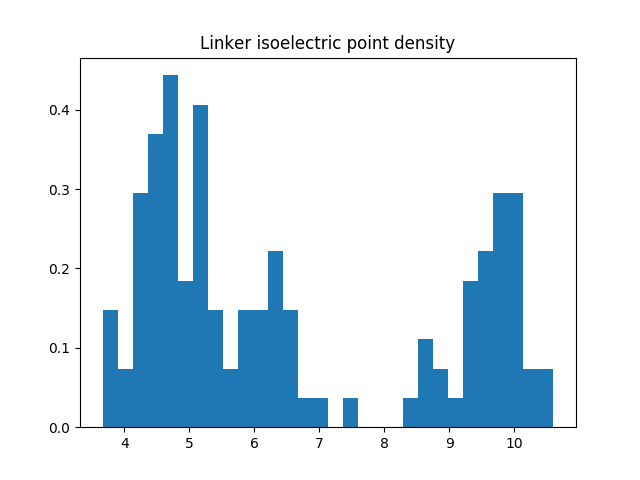
\includegraphics[width=.7\linewidth]{img/iso_density.png}
			\caption{The iso-electric point density of inter-domain regions from human
			two-domain protein kinases in the studied dataset. Two groups of proteins are
			evident, one with acidic linkers, one with basic linkers.}
			\label{fig:iso-dens}
		\end{figure}

		Au contraire, neither the percentage of charged amino acids within the non-domain
		regions, nor the linkers' GRAVY index, form distinct clusters.
		Their densities show only single local maxima.
		All linkers from the final dataset are hydrophilic, the percentage of charged residues
		averages around 0.25, hence not giving any surprising results.

	\subsecwithtoc{UMAP clustering}
	\label{res:first:umap}

		Using the first set of linkers' physicochemical attributes, the UMAP dimensionality
		reduction clustering defines three linker types.
		Throughout this thesis, the linker types will be reffered to based on the clusters'
		positioning in \cref{fig:umap}: ``L-linkers'' for the lower left cluster,
		``M-linkers'' for the middle cluster, and ``R-linkers'' for the right cluster.
		L-linkers are best characterized by their extreme length of more than 600 residues,
		R-linkers by their extremely basic iso-electric point, and M-linkers by their
		extremely acidic iso-electric point, as well as by their GRAVY index being negatively
		proportional to their percentage of charged amino acids.

		\begin{figure}
			\centering
			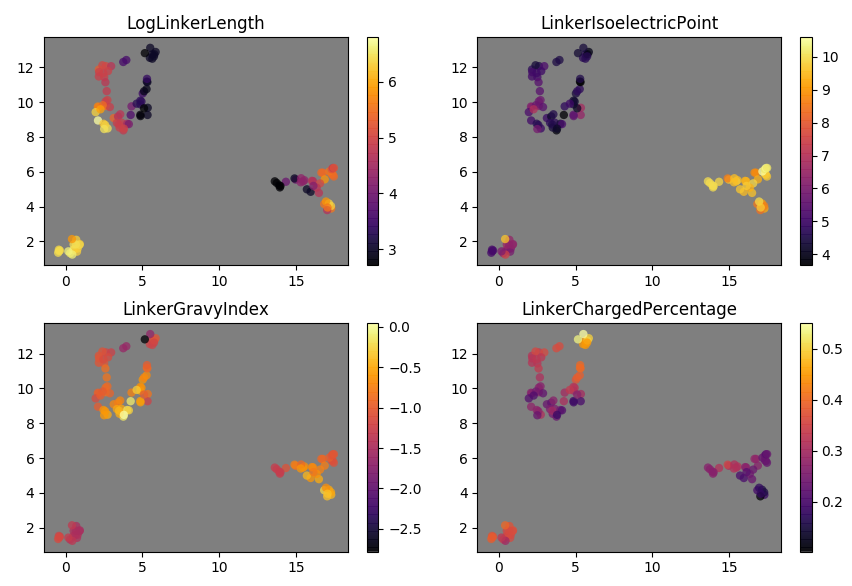
\includegraphics[width=\linewidth]{img/linker_umap.png}
			\caption{UMAP dimensionality reduction of the normalized linker attributes:
			logarithm of linker's length, iso-electric point, GRAVY index, and percentage of
			charged amino acids within the non-domain regions of human two-domain protein
			kinases. The values of the four physicochemical properties are embedded into the
			same UMAP clustering, each subfigure corresponding to one attribute.}
			\label{fig:umap}
		\end{figure}

		\begin{figure}
			\centering
			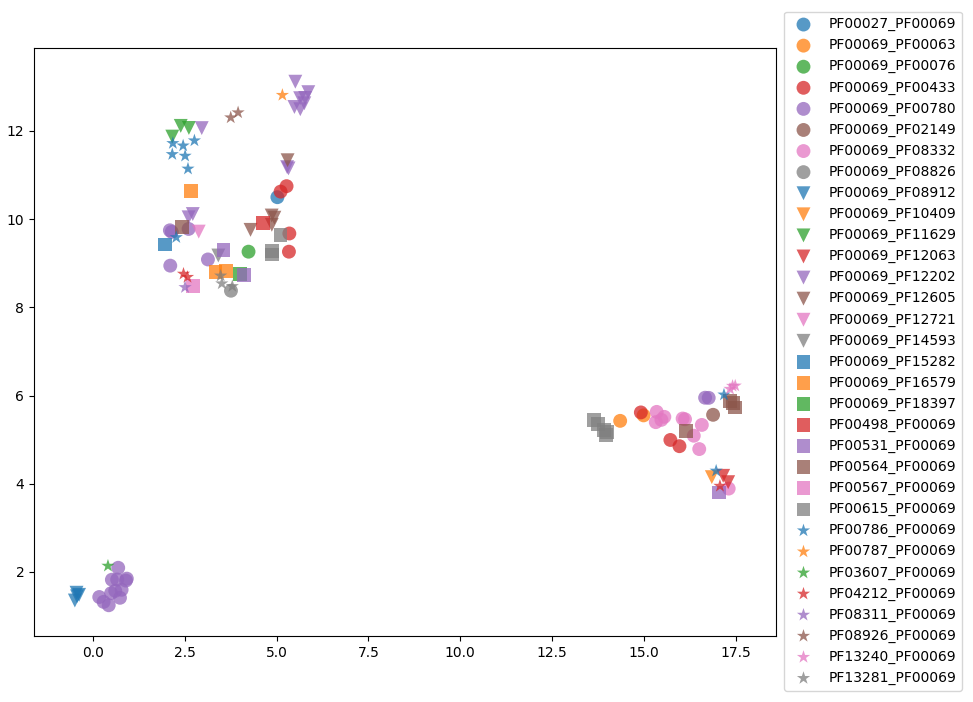
\includegraphics[width=0.9\linewidth]{img/linker_umap_arch.png}
			\caption{Architectures of the studied molecules embedded into the UMAP clustering
			of four physicochemical attributes of non-domain regions.}
			\label{fig:umap_arch}
		\end{figure}

		By embedding the architectures of the proteins from the studied dataset into the UMAP
		clustering, it is visible, that many architectures feature more than one linker type,
		as seen in \cref{fig:umap_arch}.
		Especially the architecture \texttt{PF00069\_PF00780} stands out, being endowed with
		all three linker classes.
		On the other hands, most architectures equipped with linkers from only one category
		are represented by a very narrow subset of proteins from the set of human two-domain
		protein kinases.

	\subsecwithtoc{Gene Ontology terms}
	\label{res:first:go}

		All considered proteins had at least two GO terms, one of them always being
		\texttt{GO:0005524; F:ATP binding}.
		The second most common was \texttt{GO:0004674; F:protein serine/threonine kinase
		activity}, and the third most frequent GO term was \texttt{GO:0004672; F:protein
		kinase activity}.

		However, the search for unique GO terms within both UMAP and iso-electric point
		clusterings of the non-domain regions on different GO hierarchical levels gave no
		satisfactory results, albeit discovering many GO terms exclusive for each examined
		linker group.
		These terms were namely terribly underrepresented in proteins found within the
		clusters, and no unique vocable was found spanning any whole inter-domain region
		bundle.

		There were only two GO terms standing out, regarding their proportion.
		\texttt{GO:0000287; F:magnesium ion binding} found on hierarchy level 6 is exclusive
		to the acidic linker group, as well as to the M-linkers.
		It was encountered in 12 proteins, covering 8 different architectures, including those
		having the \texttt{PF00069} domain on the N-terminus, as well as those carrying the
		protein kinase domain on the C-terminus.
		The second vocable is \texttt{GO:0005516; F:calmodulin binding} appearing on hierarchy
		level 4, being limited to the basic linker group, likewise to the R-linkers.
		Regrettably, all 10 proteins accredited with this GO term possess the same
		architecture.

	\subsecwithtoc{Enzyme Commission numbers}
	\label{res:first:ec}

		\begin{figure}
			\centering
			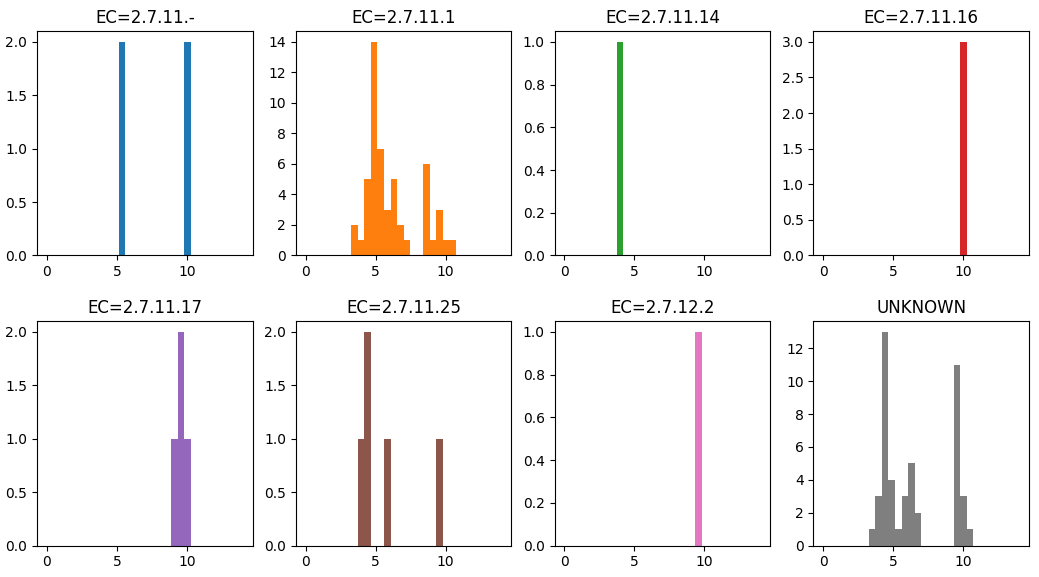
\includegraphics[width=\linewidth]{img/iso_density_ec.png}
			\caption{Occurences of EC numbers in human two-domain protein kinases. The $x$-axis
			represents the iso-electric point of the molecules' linkers.}
			\label{fig:ec}
		\end{figure}

		Out of the 117 human heterodimeric protein kinases, 70 molecules have an EC number
		assigned in the \texttt{uniprot\_reference\_proteomes.dat} file.
		For the remaining 47, the Enzyme Commission term will be reffered to as
		``\texttt{UNKNOWN}''.
		3 kinases had more than one EC number specified, some of these extra terms are
		outside of the \texttt{2.7.11 protein-serine/threonine kinases} group.
		Only 14 molecules had, however, EC classification other than \texttt{2.7.11.-},
		\texttt{2.7.11.1 non-specific serine/threonine protein kinase}, or \texttt{UNKNOWN}.

		\Cref{fig:ec} shows the distribution of the linkers' iso-electric point for each EC
		number.
		All 5 specialized EC terms are vastly underrepresented within the studied dataset, yet
		for example the \texttt{2.7.11.25 mitogen-activated protein kinase kinase kinases}
		are even present in both acidic and basic linker cluster.
		Contrarily, basic inter-domain regions seem to be specific to both \texttt{2.7.11.16
		G-protein coupled receptor kinases} and
		\texttt{2.7.11.17 Ca\textsuperscript{2+}/calmodulin-dependent protein kinases},
		nevertheless, they are not to be found in more than one architecture.

		\begin{figure}
			\centering
			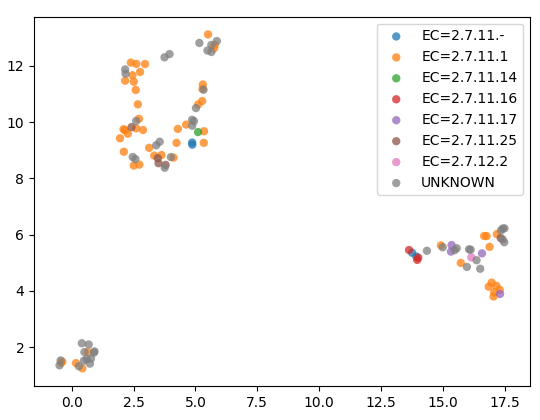
\includegraphics[width=0.8\linewidth]{img/linker_umap_ec.png}
			\caption{Embedding of the EC numbers into the UMAP dimensionality reduction
			clustering.}
			\label{fig:umap_ec}
		\end{figure}

		The inadequate representation of the EC numbers in the final dataset was also the
		reason behind the unsatisfactory results of embedding the terms into the UMAP
		dimensionality reduction clustering.
		On one hand, the numbers \texttt{2.7.11.14}, \texttt{2.7.11.16}, and
		\texttt{2.7.11.17} are specific to one of the three defined linker groups, on the
		other hand, they are not to be found in more than one architecture, as already
		mentioned above.
		In conclusion, the first set of physicochemical attributes did not provide any
		interesting results.

\secwithtoc{Second set of physicochemical attributes}
\label{res:second}

	The UMAP dimensionality reduction of the 553 physicochemical data from the AAindex
	database did not reflect the clustering of 4 physicochemical attributes described above
	at all.
	As seen in \cref{fig:aa_umap}, one small cluster of non-domain regions from human
	heterodimeric protein kinases emerges on the right side of the visualization, however,
	it contains only proteins with the same architecture \texttt{PF00069\_PF12202}.
	In the large cloud on the left side, generally, molecules with the same architecture
	create local bundles, and they only seldom mix with proteins with other
	architectures.
	Due to the lack of clearly distinguishable clusters, no GO or EC embedding was
	performed.

	\begin{figure}
		\centering
		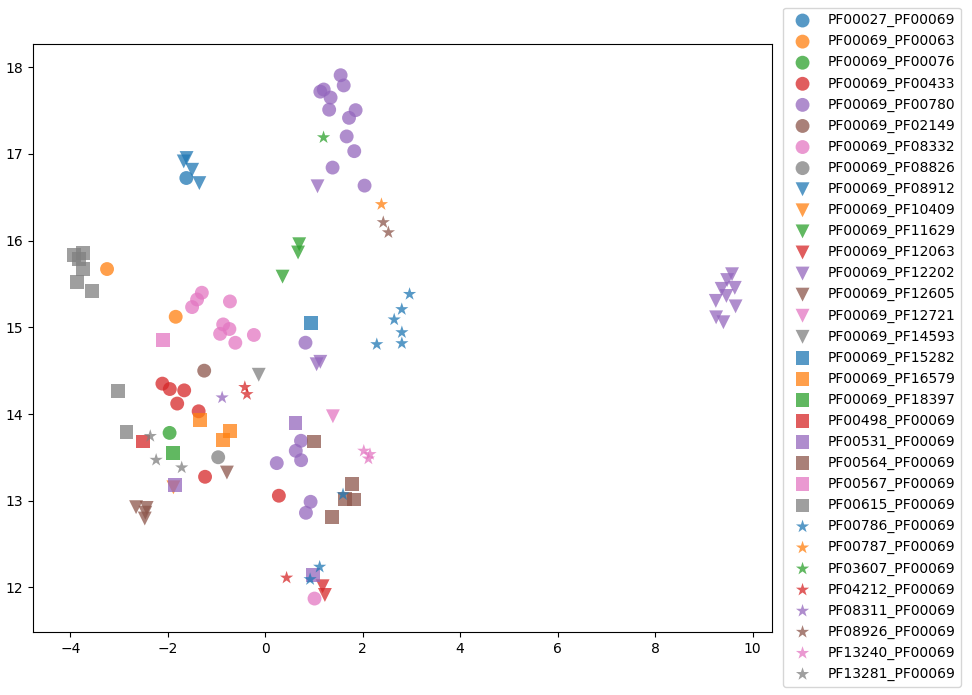
\includegraphics[width=0.9\linewidth]{img/aa_umap_arch.png}
		\caption{Architectures of the heterodimeric protein kinases embedded into the UMAP
		dimensionality reduction of 553 physicochemical properties from the AAindex database.}
		\label{fig:aa_umap}
	\end{figure}

	In conclusion, no obvious influence of non-domain regions' composition on the activity
	of human heterodimeric protein kinases was observed, as no evident clustering of the
	linkers' physicochemical properties segregating frequent GO terms or EC numbers
	belonging to different architectures was achieved.

% \chapter{More complicated chapter}
% \label{chap:math}
%
% After the reader gained sufficient knowledge to understand your problem in \cref{chap:refs}, you can jump to your own advanced material and conclusions.
%
% You will need definitions (see \cref{defn:x} below in \cref{sec:demo}), theorems (\cref{thm:y}), general mathematics, algorithms (\cref{alg:w}), and tables (\cref{tab:z})\todo{See documentation of package \texttt{booktabs} for hints on typesetting tables. As a main rule, \emph{never} draw a vertical line.}. \Cref{fig:f,fig:g} show how to make a nice figure. See \cref{fig:schema} for an example of TikZ-based diagram. Cross-referencing helps a lot to keep the necessary parts of the narrative close --- use references to the previous chapter with theory wherever it seems that the reader could have forgotten the required context.
%
% \section{Example with some mathematics}
% \label{sec:demo}
%
% \begin{defn}[Triplet]\label{defn:x}
% Given stuff $X$, $Y$ and $Z$, we will write a \emph{triplet} of the stuff as $(X,Y,Z)$.
% \end{defn}
%
% \newcommand{\Col}{\textsc{Colour}}
%
% \begin{thm}[Car coloring]\label{thm:y}
% All cars have the same color. More specifically, for any set of cars $C$, we have
% $$(\forall c_1, c_2 \in C)\:\Col(c_1) = \Col(c_2).$$
% \end{thm}
%
% \begin{proof}
% Use induction on sets of cars $C$. The statement holds trivially for $|C|\leq1$. For larger $C$, select 2 overlapping subsets of $C$ smaller than $|C|$ (thus same-colored). Overlapping cars need to have the same color as the cars outside the overlap, thus also the whole $C$ is same-colored.\todo{This is plain wrong though.}
% \end{proof}
%
% \begin{table}
% \centering
% {\footnotesize\sf
% \begin{tabular}{llrl}
% \toprule
% Column A & Column 2 & Numbers & More \\
% \midrule
% Asd & QWERTY & 123123 & -- \\
% Asd qsd 1sd & \textcolor{red}{BAD} & 234234234 & This line should be helpful. \\
% Asd & \textcolor{blue}{INTERESTING} & 123123123 & -- \\
% Asd qsd 1sd & \textcolor{violet!50}{PLAIN WEIRD} & 234234234 & -- \\
% Asd & QWERTY & 123123 & -- \\
% \addlinespace % a nice non-intrusive separator of data groups (or final table sums)
% Asd qsd 1sd & \textcolor{green!80!black}{GOOD} & 234234299 & -- \\
% Asd & NUMBER & \textbf{123123} & -- \\
% Asd qsd 1sd & DIFFERENT & 234234234 & (no data) \\
% \bottomrule
% \end{tabular}}
% \caption{An example table. Table caption should clearly explain how to interpret the data in the table. Use some visual guide, such as boldface or color coding, to highlight the most important results (e.g., comparison winners).}
% \label{tab:z}
% \end{table}
%
% \begin{figure}
% \centering
% \includegraphics[width=.6\linewidth]{img/ukazka-obr02.pdf}
% \caption{A figure with a plot, not entirely related to anything. If you copy the figures from anywhere, always refer to the original author, ideally by citation (if possible). In particular, this picture --- and many others, also a lot of surrounding code --- was taken from the example bachelor thesis of MFF, originally created by Martin Mareš and others.}
% \label{fig:g}
% \end{figure}
%
% \begin{figure}
% \centering
% \tikzstyle{box}=[rectangle,draw,rounded corners=0.5ex,fill=green!10]
% \begin{tikzpicture}[thick,font=\sf\scriptsize]
% \node[box,rotate=45] (a) {A test.};
% \node[] (b) at (4,0) {Node with no border!};
% \node[circle,draw,dashed,fill=yellow!20, text width=6em, align=center] (c) at (0,4) {Ugly yellow node.\\Is this the Sun?};
% \node[box, right=1cm of c] (d) {Math: $X=\sqrt{\frac{y}{z}}$};
% \draw[->](a) to (b);
% \draw[->](a) to[bend left=30] node[midway,sloped,anchor=north] {flow flows} (c);
% \draw[->>>,dotted](b) to[bend right=30] (d);
% \draw[ultra thick](c) to (d);
%
% \end{tikzpicture}
% \caption{An example diagram typeset with TikZ.}
% \label{fig:schema}
% \end{figure}
%
% \begin{algorithm}
% \begin{algorithmic}
% \Function{ExecuteWithHighProbability}{$A$}
% 	\State $r \gets$ a random number between $0$ and $1$
% 	\State $\varepsilon \gets 0.0000000000000000000000000000000000000042$
% 	\If{$r\geq\varepsilon$}
% 		\State execute $A$ \Comment{We discard the return value}
% 	\Else
% 		\State print: \texttt{Not today, sorry.}
% 	\EndIf
% \EndFunction
% \end{algorithmic}
% \caption{Algorithm that executes an action with high probability. Do not care about formal semantics in the pseudocode --- semicolons, types, correct function call parameters and similar nonsense from `realistic' languages can be safely omitted. Instead make sure that the intuition behind (and perhaps some hints about its correctness or various corner cases) can be seen as easily as possible.}
% \label{alg:w}
% \end{algorithm}
%
% \section{Extra typesetting hints}
%
% Do not overuse text formatting for highlighting various more or less parts of your sentences; if an idea cannot be communicated without formatting, the sentence probably needs rewriting anyway.
%
% Most importantly, do \underline{not} overuse bold text, which is designed to literally \textbf{shine from the page} to be the first thing that catches the eye of the reader. More precisely, use bold text only for `navigation' elements that need to be seen first, such as headings, list item names, and figure numbers.
%
% Use underline only in dire necessity, such as in the previous paragraph where it was inevitable to ensure that the reader remembers to never typeset boldface text manually again.
%
% Use \emph{emphasis} to highlight the first occurrences of important terms that the reader should notice. The feeling the emphasis produces is, roughly, ``Oh my --- what a nicely slanted word! Surely I expect it be important for the rest of the thesis!''
%
% Finally, never draw a vertical line (e.g., in a table or around figures), ever. Vertical lines outside of the figures are ugly.

\chapter{Discussion}
\label{discussion}

The length and amino acid composition of non-domain regions can be crucial for the
regulation of multi-domain proteins' activity, including
PKs~\cite{gogl2019disordered, vigil2004conformational}.
However, to our knowledge, the influence of the linkers' composition on the overall
protein function has not been described \emph{in general} yet.
This thesis tried to address this issue by selecting a dataset of evolutionarily related
multi-domain proteins containing a PK domain, clustering these molecules based on the
physicochemical attributes of their inter-domain regions, and by identifying GO terms and
EC numbers specific to the detected clusters of proteins with various architectures.

Even though it was possible to divide proteins from the studied dataset into three groups
based on the clusters visible in the UMAP representation of the 4-dimensional space of
the linkers' normalized physicochemical characters, no frequent functional annotation
terms could characterize the defined clusters.
There may be several reasons for the lack of success of the designed method.
For example, there may really not be any overall influence of the inter-domain regions'
composition on the function of two-domain PKs.
However, based on the literature search presented above, this proposition seems rather
improbable~\cite{winkler1977tomato, van1997linker, ikebe1998hinge, robinson1998optimizing,
rice1999structural, gokhale2000role, case2000role, pufall2002autoinhibitory,
khalil2008kinesin, hariharan2009insights, smock2010interdomain, liu2010molecular,
shastry2010neck, ma2011dynamic, cyrus2011impact, kalodimos2011nmr, pohane2015modulation,
klement2015effect, rozycki2017length, jakubec2018widespread, gogl2019disordered}.

The narrow dataset may be a significant problem.
In a sample of large size, more information is available; on the other hand, false
presumptions may be concluded from a small sample generating the
observations~\cite{tanaka1987big, hua2005optimal}.
In the studied dataset, 32 different architectures were present within the 117 molecules.
Proteins with the same architecture are frequently related, both evolutionarily and
functionally~\cite{vogel2004structure, hegyi2001annotation, bashton2002geometry}, and the
linkers may introduce new structural features~\cite{papaleo2016role}, thus enhancing the
functionality.
With 3.65625 proteins per architecture on average, no robust conclusion can be made on how
the composition of the linkers affects the behavior of these molecules.

Furthermore, both functional annotation services, GO and EC, have drawbacks regarding
their completeness and homogeneity.
For instance, \citet{gaudet2017gene} claim that the GO is biased and unevenly incomplete.
The GO database is a reflection of primary literature~\cite{gene2004gene}, therefore, less
studied areas are inadequately represented in the GO.
On the other hand, more comprehensively covered parts of the GO are not flawless either,
as they can provide contradictory information which can be caused, for example, by
differences in experimental conditions of comparable
research~\cite{hass2004response, mason2005multiple}.

Within the studied 117 human two-domain PKs, a total of 1,982 GO annotations were fetched
from the UPR.dat file, peaking at 69 terms assigned to a single protein, namely the
\texttt{AAPK1\_HUMAN} PK.
These include even the GO terms from the same hierarchy.
For example, it is possible to reach \texttt{GO:0008610; lipid biosynthetic process} by
recursively applying the transitive relationship ``\texttt{is\_a}'' on
\texttt{GO:0045542; positive regulation of cholesterol biosynthetic process}, which are
both explicitly mentioned in the \texttt{uniprot\_reference\_proteomes.dat} file.
Furthermore, the same protein is classified as \texttt{2.7.11.1 non-specific
serine/threonine protein kinase}; however, at the same time, has the specific EC numbers
\texttt{2.7.11.26}, \texttt{2.7.11.27}, and \texttt{2.7.11.31} assigned to it as well.

To be assigned an EC number, there must be a direct experimental evidence that the
proposed enzyme actually catalyses the claimed reaction~\cite{mcdonald2014fifty}.
60 proteins from the studied dataset were described as \texttt{2.7.11.1 non-specific
serine/threonine protein kinase}, meaning that these PKs are either non-specific,
or their specificity has not been analyzed to
date\footnote{\url{https://www.brenda-enzymes.org/enzyme.php?ecno=2.7.11.1}}.
%Neither of these possibilities are favorable regarding the goal of this thesis.
The strict nature of the EC, as well as the excessiveness of the GO combined with
insufficient amount of research could be overcome by measuring similarities of the GO
terms~\cite{li2010effectively, zhao2018gogo} within the protein clusters instead of
enforcing their absolute exclusion.

Furthermore, it may be desirable to employ a more stable method than UMAP to produce a
significant outcome.
The low-dimensional representation generated by UMAP is dependent on the
choice of several
hyperparameters\footnote{\url{https://umap-learn.readthedocs.io/en/latest/parameters.html}}.
Besides, UMAP is a stochastic algorithm, and exact reproduction of the results is only
possible by fixing a random seed
state\footnote{\url{https://umap-learn.readthedocs.io/en/latest/reproducibility.html}}.
The observed linker types are therefore determined by UMAP parametrization.

The elucidation of the effect of the linkers' composition on protein activity could
improve our ability to predict the function of multi-domain proteins, but further
research is needed to disclose the presented problem.
Throughout this thesis, only rough and averaged characteristics of the whole
linkers were considered.
In reality, only a couple of particular residues may have an influence on the protein
activity, the rest of them may be unimportant.
The herein proposed method is not capable of resolving such residues.

% The drafted strategy applied in this thesis could be improved in future work by taking
% into account more two-domain PKs, and by implementing similarity measures of GO terms to
% condensate akin vocables, hence reducing the immensely detailed nature of the GO database.

\chapwithtoc{Conclusion}
\label{conclusion}

Based on the performed research, this thesis did not show any general influence of the
non-domain regions' composition on the performance of human two-domain protein kinases.
The poorly chosen dataset together with the incompleteness and uninformativeness of the
GO terms and EC numbers contributed to the negative result.

However, with respect to the known \emph{open-world assumption}, not observed does not
mean it is not there.
The exposure of the effect of linkers' composition on protein activity could improve our
ability to predict the function of multi-domain proteins, but further research is needed
to disclose the presented problem.
The drafted strategy applied in this thesis could be improved in future work by taking
into account more two-domain protein kinases, and by implementing similarity measures of
GO terms to condensate akin vocables, hence reducing the immensely detailed nature of the
Gene Ontology database.
Yet, success cannot be guaranteed.

\include{bibliography}

%\appendix

% if your attachments are complicated, describe them in a separate appendix
%\include{attachments}

\openright
\end{document}
